\title{{\sc qvort}\\
{\normalsize A quantised vortex code}}
\author{\normalsize
        Andrew Baggaley\\
        \normalsize  School of Mathematics and Statistics\\
        \normalsize  Newcastle Univeristy\\
        {\normalsize  U.K.}\\
        \normalsize   a.w.baggaley@gmail.com
}
\date{\normalsize   \today}

\documentclass[12pt]{article}
\usepackage{natbib}
\usepackage{graphicx}
\usepackage{hyperref}
\newcommand{\bs}{\mathbf{s}}
\newcommand{\br}{\mathbf{r}}
\newcommand{\bu}{\mathbf{u}}
\newcommand{\appsection}[1]{\let\oldthesection\thesection
  \renewcommand{\thesection}{Appendix \oldthesection}
  \section{#1}\let\thesection\oldthesection}
\begin{document}
\maketitle
\pagestyle{plain}
\pagenumbering{roman}
\tableofcontents
\newpage
\clearpage
\pagenumbering{arabic}
\begin{figure}
  \begin{center}
    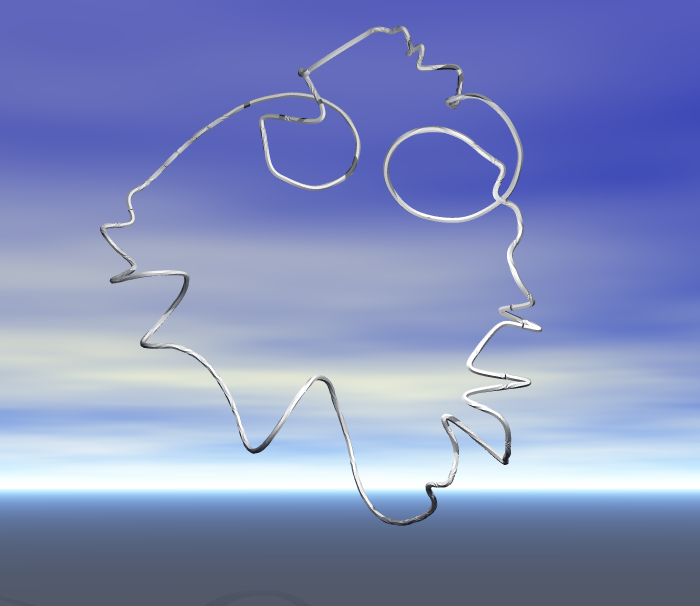
\includegraphics[scale=0.3]{./fig/header.png}%
    \caption{A 3D rendering of a vortex filament with wave perturbations, outputted from the {\sc{qvort}} code (using the bryce\_out.m script) and then rendered using the Bryce software package}
  \end{center}
\end{figure}
\section{Introduction}\label{Sec:int}
  Welcome to the documentation for the {\sc{qvort}} quantised vortex code.
  The code is written in well commented Fortran, arranged in a modular structure.
  The primary aim of this documentation is to highlight which module(s) are involved in the various sequences of the code, 
  and also the parameters which can be set in the {\it run.in} file.
  To run {\sc qvort} you need to be on a {\it UNIX}-type system ({\it Make} and {\it bash} are heavily used) with a Fortran compiler.
  All the Fortran code can be found in the directory {\it src}.
  MATLAB is used for post-processing, although it is probably very straightforward to convert the MATLAB scripts (found in {\it bin}) to work with {\it Octave}, freely available under the GNU license.
  Please do not hesitate to contact with any queries, or if you are interested in helping to further develop the code.
\section{Boundary conditions}
 AT present the code can be run with 3 different boundary conditions all of which apply to a cube with a variable size which can be set as a runtime parameter.
These are open, periodic or reflective boundaries.
If running with open boundaries the box plays no role and the filaments can move freely in space, the box size is simply used as a guide by the plotting routines.
Periodic boundaries mean that if a filament leaves one side of the box it wil re-enter on the opposite side.
Whilst this is appealing in order to investigate the properties of a the vortices in the box it does not come without some compromises.
Firstly the energy diagnostic is no longer valid, and its results should not be used.
Secondly in order to keep the velocity field continuous an extra 27 permutations of the field are required, slowing the code down considerably.
Finally one can impose reflective boundaries using the method of images in which mirror vortices are used at each of the boundaries, again significantly increasing the workload.
\section{Equations}\label{Sec:eqn}
  The {\sc qvort} code is a vortex-filament code, a technique pioneerd by Schwarz in the early 1980s. 
  Each line-vortex in the system is discretised into a number of points which are evolved according to an equation of motion.
  Points along the line are added (or removed) if the vortex is stretched (or compressed).
  If any two lines become very close (a distance less than the separation along the line) then the filaments reconnect, changing the topology of the system.  
  More precisely we define our vortex filament as a three dimensional curve $\bs=\bs(\xi,t)$.
  Here $\xi$ represents arc-lengths and $t$ is time.
  We can construct the tangent vector $\bs'$, then normal vector, $\bs''$,
  and the binormal vector, $\bs' \times \bs''$ by taking numerical derivatives.
  Note $\bs'=d \bs/d\xi$, and so on.
  We denote the velocity at a point $\bs$ as $\bu(\bs)$ and consider the velocity field to be made up of two parts,
  \begin{equation} 
     \bu=\bu_\mathrm{s}+\bu_\mathrm{n},
  \end{equation} 
  where $\bu_\mathrm{s}$ is the superfluid component of the velocity field (i.e. motion induced by vortices),
  and $\bu_\mathrm{n}$ is the normal fluid component.
  In the code there are various options for both the normal and superfluid components.
  For the superfluid component one can choose between the local induction approximation (LIA),
  \begin{equation}\label{Eq:LIA}
    \bu_\mathrm{s}=\beta \bs' \times \bs'', \qquad \beta=\frac{\Gamma}{4\pi} \ln \left( \frac{R}{a} \right),
  \end{equation} 
  where $\Gamma$ is the quantum of circulation (a parameter which can be set in {\it run.in}), 
  $R$ is the radius of curvature ($1/|\bs''|$), and $a$ is the vortex core size (fixed $10^{-8}$cm).
  We note that the time per iteration with this method scales like ${\cal O}(N)$, where $N$ is the total
  number of particles in the simulation.

  A second option is to solve the de-singulised Biot-Savart integral,
  \begin{equation}\label{Eq:BS}
    \bu_\mathrm{s}=\beta' \bs' \times \bs''+ \frac{\Gamma}{4\pi} \int_{\ell'} \frac{(\bs-\br)\times d\bs}{|\bs-\br|^3},
    \qquad \beta'=\frac{\Gamma}{4\pi} \ln \left( \frac{\sqrt{\ell_{i}\ell_{i-1}}}{a}\right).
  \end{equation}
  $\ell'$ represents the full system with the local region around the point of interest removed (to avoid division by 0).
  This local contribution enters back in as a binormal vector with a magnitude affected by the size of local region $\ell_i$/$\ell_{i-1}$.
  Whilst a more realistic scheme the downside of using the full integral comes in the scaling of the time per iteration with $N$, which is quadratic (${\cal O}(N^2)$).
      
  The current options for the normal fluid are zero, $\bs_\mathrm{n}=0.$, a constant $x$-flow, 
  $\bu_\mathrm{n}=(\mathrm{const},0,0),$ the ABC flow,
  \begin{equation} 
    \bu_\mathrm{n}=
  \end{equation}
  We can also set a constant flow in the $x$-direction, $\bu_\mathrm{n}(1)=\mathrm{const.}$ or use the KS model to give a synthetic turbulent velocity field, using a summation of random Fourier-modes with an imposed Energy spectrum.
  These two velocities combined together to give the total equation of motion
  \begin{equation}
    \frac{d \bs}{dt}=\bu_\mathrm{s}+\alpha \bs' \times (\bu_\mathrm{n}-\bu_\mathrm{s})
    +\alpha' \bs' \times \left[ \bs' \times (\bu_\mathrm{n}-\bu_\mathrm{s})\right]
  \end{equation}  
\section{Numerical schemes}\label{Sec:num}
  At a particular particle on a filament, with position $\bs_i$, define the distance to the particle in-front ($\bs_{i+1}$)
  as $\ell_{i+1}$ and the distance to the particle behind ($\bs_{i-1}$) as $\ell_{i-1}$.
  By in-front/behind we refer to the particles next/previous along the filament.
  We can construct finite difference approximations to the first and second derivatives by taking Taylor's series expansions.
  The resulting forms are as follows,
  \begin{equation}
    \frac{d \bs_i}{d \xi}=\frac{\ell_{i-1}\bs_{i+1}+(\ell_{i+1}-\ell_{i-1})\bs_i+\ell_{i+1}\bs_{i-1}}
    {2\ell_{i+1}\ell_{i-1}}+{\cal O}(\ell^2),
  \end{equation}
  \begin{equation}
    \frac{d^2 \bs_i}{d \xi}^2=\frac{2\bs_{i+1}}{\ell_{i+1}(\ell_{i+1}+\ell_{i-1})}-\frac{2\bs_i}{\ell_{i+1}\ell_{i-1}}+\frac{2\bs_{i-1}}{\ell_{i-1}(\ell_{i+1}+\ell_{i-1})}+{\cal O}(\ell^2).
  \end{equation}
  We must also use some numerical scheme to integrate in time. Due to the cost of calculating the velocity field at each point (scales with $N^2$ in the Biot-Savart case) it is very intensive to use a Runge-Kutta type scheme. 
Therefore we use the $3^rd$ order Adams-Bashforth method where the evolution of each particle at a point $\mathbf{x}_i$ is given by:
\begin{equation}
  \mathbf{s}_i^{n+1}=\mathbf{s}_i^{n}+h\mathbf{u_i}^n.
\end{equation}
We denote $h$ as our time-step, and note that this is controlled by the maximum resolution discussed below.
\subsection{Line algorithms}
  If the separation between two points on the filament becomes two large we must introduce a new point in order to maintain the resolution along the filament.
As the evolution equation for a vortex filament is sensitive to the local curvature linear interpolation is not a good idea.
A way to keep the curvature constant is to use the following algorithm,
\begin{equation}
\bs_{i'}=\frac{1}{2}(\bs_i+\bs_{i+1})+\left( \sqrt{R^2_{i'}-\frac{1}{4}\ell_i^2}-R_{i'} \right)\frac{\bs_{i'}^{''}}{|\bs_{i'}^{''}|},
\end{equation}
where $\bs_{i'}$ is the position of the point introduced if the separation between the points $\bs_{i}$ and $\bs_{i+1}$  becomes greater than some threshold $\delta$, which we note is the minimum resolution.
Note, 
\begin{equation}
\bs^{''}_{i'}=\frac{\bs_i+\bs_{i+1}}{2},
\end{equation}
and $R_{i'}=|\bs_{i'}^{''}|^{-1}$.
If the separation between two points becomes less than $\delta/2$ then we remove a point to ensure that we never have a maximum resolution greater than $\delta/2$. 

As discussed above our time-step $h$ is controlled by the size of $\delta$ in the following way.

At present the time-step is set manually in the code, however you will not be able to run the code and will receive a fatal error.

\section{Running the code}
To run the code you must first compile it using the following commands under a linux/unix system
\begin{verbatim}
make
\end{verbatim}
ensure that there is a data directory, if not create with the following command,
\begin{verbatim}
mkdir ./data
\end{verbatim}
copy an example run file from the directory examples, for example
\begin{verbatim}
cp ./examples/single_loop.in ./run.in
\end{verbatim}
the code then be run with the following command
\begin{verbatim}
./run.sh
\end{verbatim}
the run script can take a variety of options, if interested run the command
\begin{verbatim}
./run.sh -h
\end{verbatim}
for example the following command will restart the code if possible
\begin{verbatim}
./run.sh -r
\end{verbatim}
\subsection{Editing the run.in file}
In this next section we provide documentation of all the possible arguments that can be set in the run.in file.
This is split into two sections, the essential parameters which must be set for the code to run, and optional parameters. 
\subsubsection{Essential parameters}
\begin{center}
\begin{tabular}{|c|c|c|}
    \hline
parameter & description & arguments\\
    \hline
nsteps   & the number of time-steps to use & positive (large) integer \\
shots   & how often to print to file & positive integer \\
shots   & how often to print to file & positive integer \\
pcount   &  \# points are used in the initial conditions & positive integer \\ 
dt & the time-step - if too large code will not run & positive real  \\
delta & the resolution (spacing of points on filaments) & positive real \\
box\_size & the length of the side of the cube we run in & positive real \\
velocity & how we calculate the velocity field & LIA, BS, Tree \\
initf & our initial configuration & single\_loop \\
      &                           & single\_line \\
      &                           & random\_loops \\
      &                           & crow \\

      &                           & leap-frog \\
      &                           & lined\_filaments \\
      &                           & colliding\_loops \\
      &                           & kivotedes \\
      &                           & cardoid \\
      &                           & wave\_loop \\
      &                           & wave\_line \\
      &                           & line\_motion \\
      &                           & tangle \\
boundary & the boundary conditions & open, periodic, mirror\\
    \hline
\end{tabular}
\end{center}
\subsubsection{Optional parameters}
These all have default values (shown in brackets) which, in general, turn the specific feature off.
\begin{flushleft}
\begin{tabular}{|c|c|c|}
    \hline
parameter & description & arguments\\
    \hline
line\_count & how many lines or loops for certain initf & positive integer(1)\\
quant\_circ & quantum of circulation & positive real(0.00097)\\
mesh\_size & print normal/superfluid velocity on a mesh& integer (0) \\
tree\_theta & opening angle if using tree algorithms & positive integer(0)\\
tree\_print & print the tree mesh to file & T/F (F)\\
binary\_print & print the files as binary data & T/F (T) \\
curv\_hist & binned curvature information for histogram & T/F (F) \\
mirror\_print & print the image vortices to file & T/F (F)\\
normal\_velocity & normal fluid velocity field & zero (zero) \\
                 &                           & xflow \\
                 &                           & ABC \\
                 &                           & KS \\

normal\_fluid\_cutoff & turn off the normal fluid at certain $t$ & positive real (100.) \\
alpha & mutual friction coefficients & two reals (0. 0.) \\
quasi\_pcount & number of particles in the code & integer (0) \\
particle\_type & the type of particles & fluid, inertial \\
initg & the initial configuration of the particles & random, one-side, pairs\\
force & do we want forcing in the code & off (off)\\
                 &                           & top\_boundary \\
                 &                           & box\_shake \\
                 &                           & delta\_corr \\
force\_amp & the amplitude of the forcing (in terms of $\delta$)& real (0.)\\
force\_freq & the forcing frequency & real (0.)\\
special\_dump & dump the filament information at a specific $t$& real (0.)\\
wave\_count & for wave\_line/loop initial condition & integer (1)\\
wave\_slope & for wave\_line/loop initial condition & real (-1.5)\\
wave\_amp & for wave\_line/loop initial condition & real (10)\\
wave\_type & for wave\_line/loop initial condition & planar, helical (planar)\\
    \hline
\end{tabular}
\end{flushleft}
Final section on stiff ode solver
\end{document}

